\chapter{Chapter 1}
    \section{Lateritic Weathering – Theoretical Formation Mechanism. Illustration of the Chua Hoi Son Outcrop}

        \subsection{Lateritic Weathering}

        \hspace*{0.6cm}Lateritic weathering is a complex process that involves multiple stages and diverse geochemical reactions. The formation of laterite is controlled by several factors, including climate, the composition of the parent rock, and the degree of leaching. The accumulation of iron and aluminum oxides and hydroxides play a crucial role in producing the distinctive reddish coloration and characteristic structure of laterite.

        \textbf{Illustration of Outcrop Point 2: Chua Hoi Son}

        \textbf{Coordinates:} 10°52'33''N - 106°50'25''E

        \textbf{Time:} 8:15–8:45 AM, October 31, 2025

        \textbf{Weather:} Hot, partly cloudy

        \textbf{Description:}
        \begin{itemize}
            \item \textbf{Structure of the outcrop:} Formed from chemical sedimentary processes:
            \begin{itemize}
                \item Composed of parent rock (shale, partly basalt, …)
                \item Gently sloping terrain
                \item Suitable pH level
                \item Groundwater level fluctuates slightly, about 3–4 m between rainy and dry seasons
                \item Sufficiently long weathering duration, forming minerals such as Fe\textsuperscript{2+}, Fe\textsuperscript{3+}, Mn\textsuperscript{2+}, Al\textsuperscript{3+}, …
            \end{itemize}
            \item At the Chua Hoi Son site, laterite belonging to the Thu Duc Formation can be observed. It has a brown to reddish-brown color, unevenly distributed, with large, solid, irregular pores that are not saturated with water. When completely weathered, the laterite becomes very hard. The mineral composition includes clay, sand, and oxides. The unweathered part is softer, and when scraped, produces reddish-brown sand.
        \end{itemize}

        \subsection{Formation Mechanism of Laterite}

        \begin{itemize}
            \item \textbf{Environmental conditions:} Suitable pH level (In tropical regions).
            \item \textbf{Initial conditions:} Parent rock must contain cations Fe\textsuperscript{2+}, Fe\textsuperscript{3+}, Mg\textsuperscript{2+}, Al\textsuperscript{3+}
            \item A groundwater table that is neither deep nor shallow.
            \item \textbf{Time condition:} Sufficiently long accumulation.
            \item When underground, Laterite rock is still soft. After being brought to the surface and exposed to the air, the rock rapidly and irreversibly hardens. The weathered part is bluish-gray and hard; the unweathered part is soft and friable, containing red, fine sand within its pores.
        \end{itemize}

        \begin{figure}[H]
            \centering
            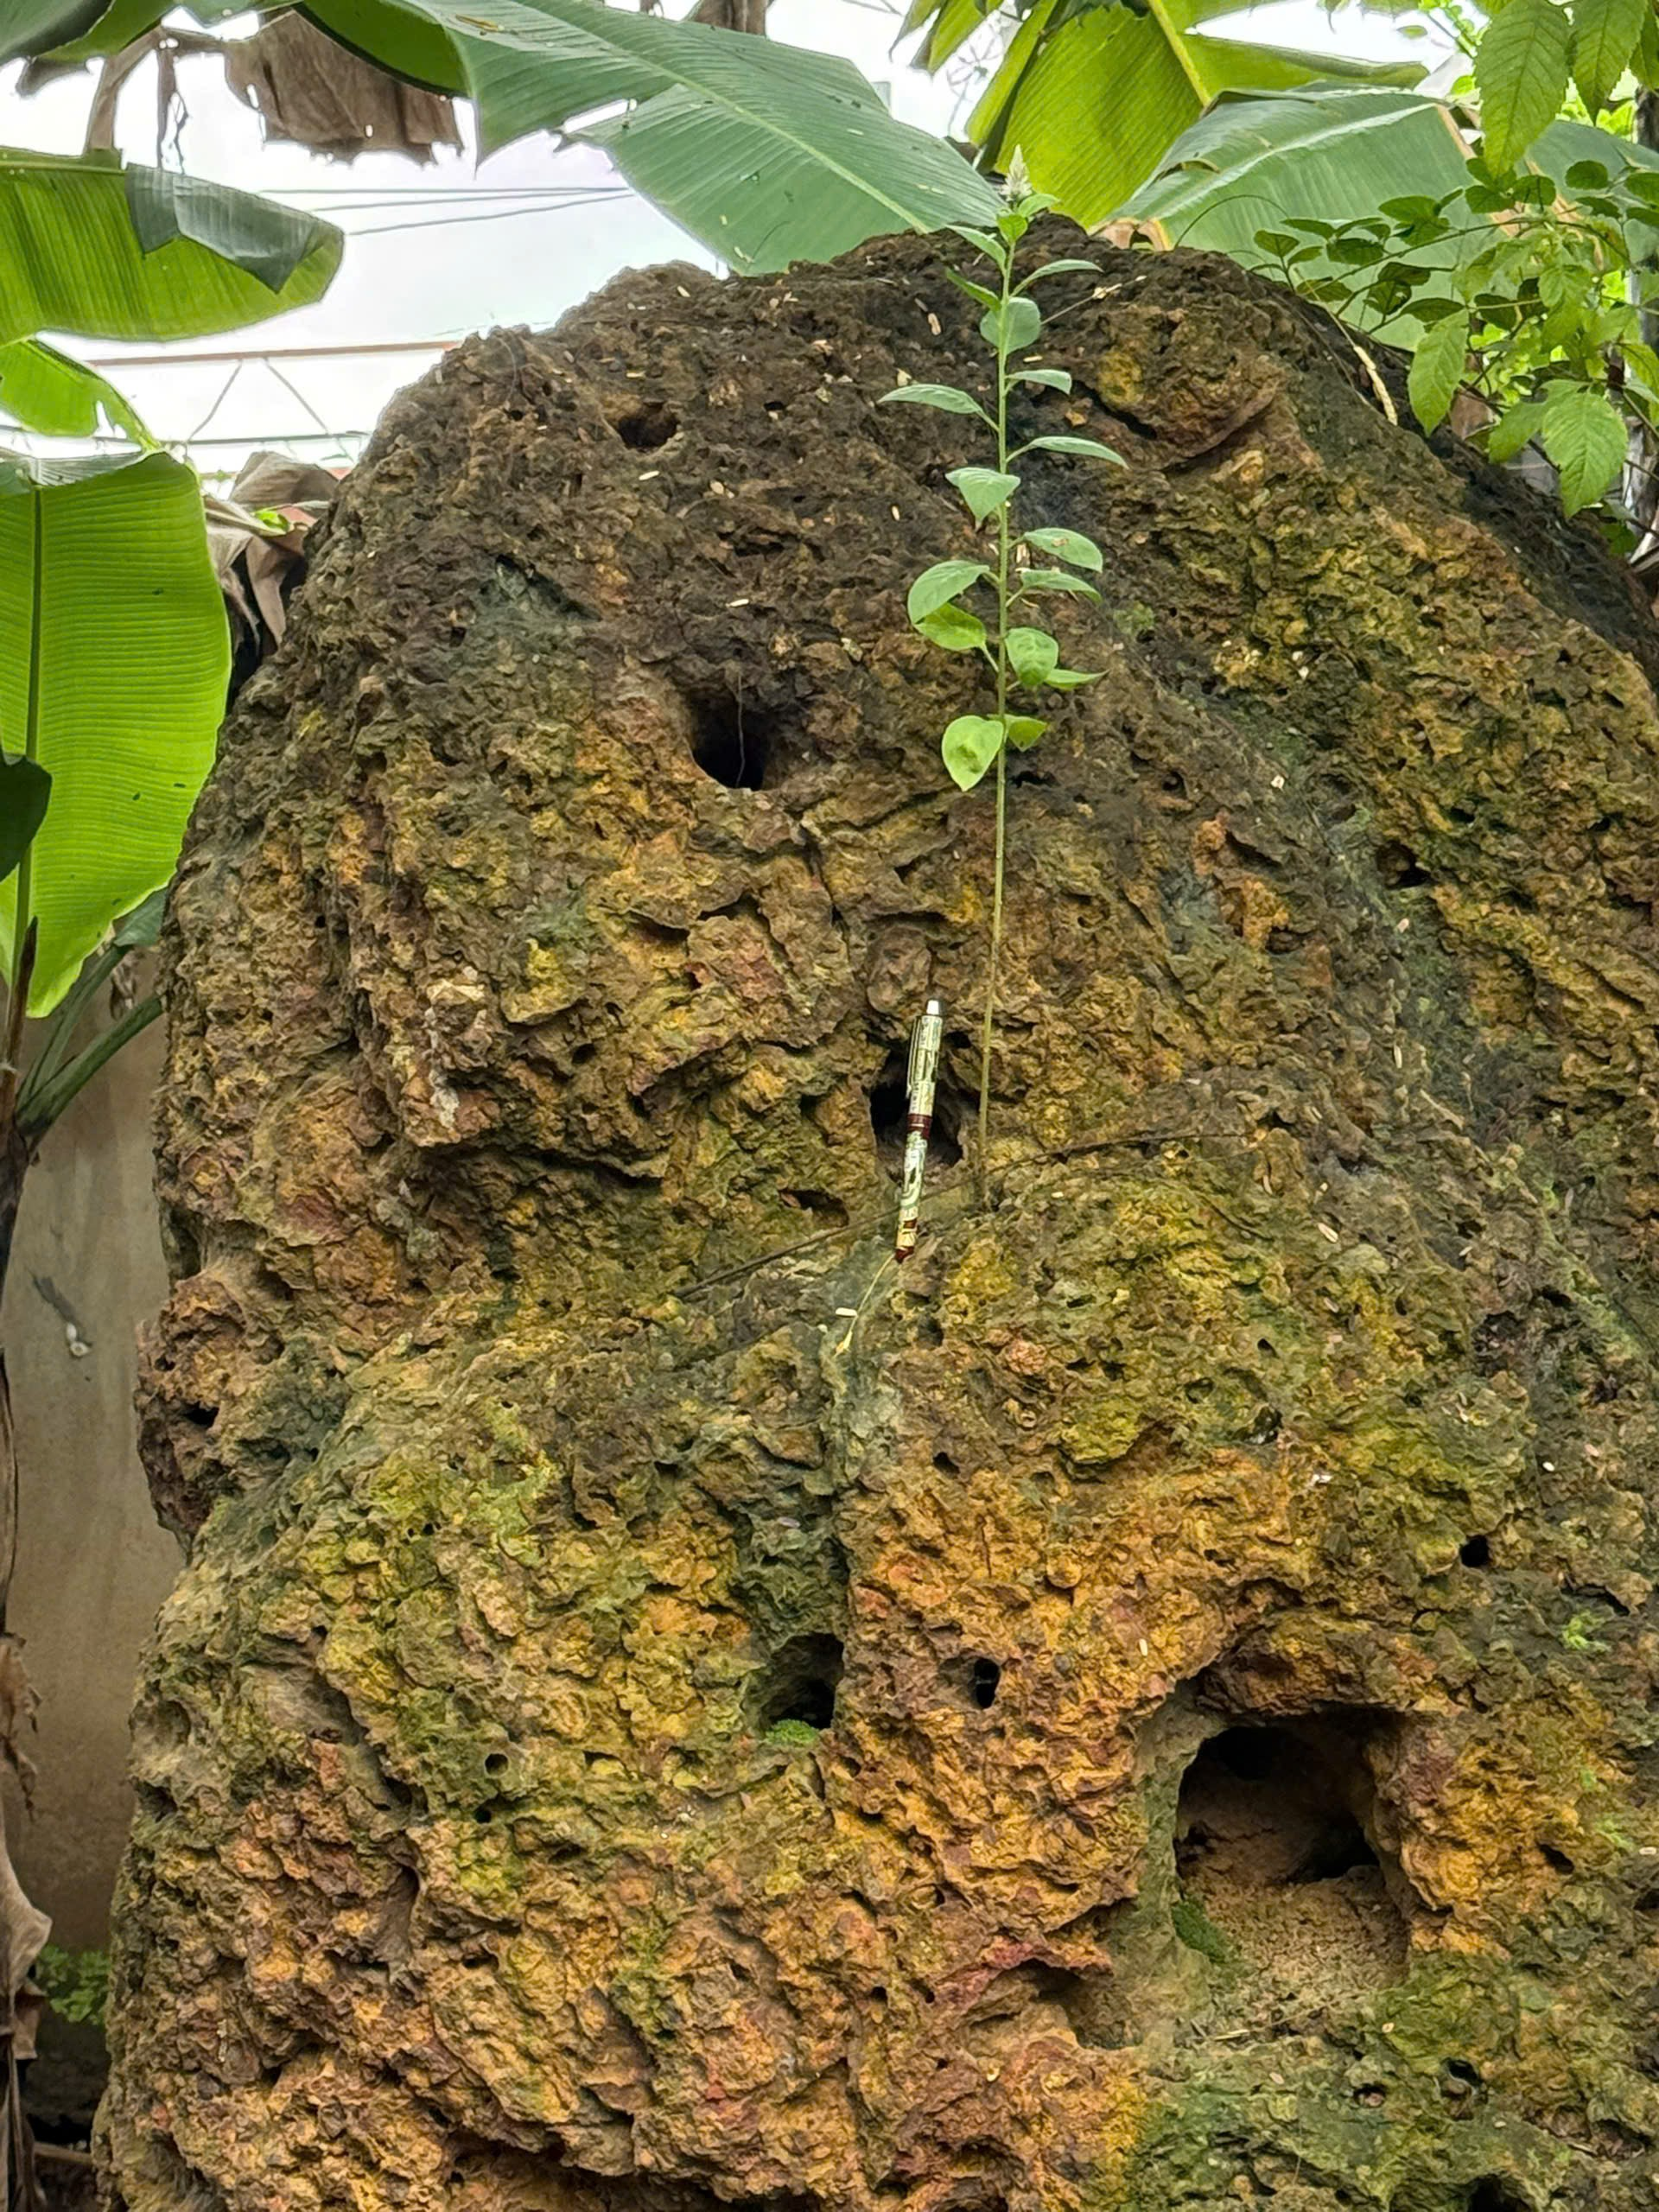
\includegraphics[width=0.8\textwidth]{pictures/chapter1/c1_p1_Laterite.png}
            \caption{Laterite rock at Hoi Son Pagoda}
            \label{fig:laterite}
        \end{figure}

        \section{Erosion – Coastal Shoreline Processes, Illustration of the Estuarine Area}

        \hspace*{0.6cm}Coastal erosion and shoreline degradation are complex processes influenced by both natural and human factors. These processes can cause significant changes in coastal topography and environment. Coastal erosion and shoreline degradation result from the combination of natural and anthropogenic factors.

        Understanding these processes is crucial for effectively implementing coastal protection and management measures, aiming to minimize damage and preserve the coastal environment.

        \textbf{Illustration of Outcrop Point 6: Estuarine Area}

        \textbf{Coordinates:} 10°23'23''N - 107°9'17''E

        \textbf{Time:} 7:00–8:00 AM, November 1, 2025

        \textbf{Weather:} Hot, partly cloudy

        \textbf{Description:}
        \begin{itemize}
            \item \textbf{Coastal wave erosion:} Mixed with shells, black sand, and quartz. Water carries these materials along. As the water recedes, the materials move with the current and deposit elsewhere, causing erosion on one side and deposition on the other.
            \item \textbf{Water deposition:} Refers to rainwater settling in the lowest areas.
            \item \textbf{Mangrove forests at estuaries:} Trees in Vietnam's mangrove forests have stilted roots that rise above the ground, which are thick, strong, and dense. Most are plants with prop roots, such as Rhizophora, Sonneratia (Su), Bruguiera (VVet), Melaleuca (Tram), and Avicennia (MMam).
            \item \textbf{Formation of sediments by wave ripples.}
        \end{itemize}

        \subsubsection*{Sediment Formation Process:}
        \begin{itemize}
            \item \textbf{Sediment deposition:} Ripples on the sea or river surface transport and accumulate particles such as sand, mud, and biological debris in layers. These layers often form wavy patterns due to the action of currents or waves.
            \item \textbf{Compaction and alteration:} Over time, the sediment layers are compacted by gravity and by the deposition of new layers on top. This process causes changes in the structure and texture of the particles, making them stick together to form sedimentary rock.
            \item \textbf{Lithification:} Dissolved minerals in groundwater penetrate the sediment layers and precipitate, binding the particles together. This process, called lithification, transforms the sediment layers into solid sedimentary rock.
        \end{itemize}

        \section{Magma Eruption Process – Rhyolite of the Nha Trang Formation. Illustrated in Vung Tau}

        \hspace*{0.6cm}The process of magma eruption and the formation of rhyolite in the Nha Trang Formation is a complex one, involving the generation of magma from the Earth's crust, accumulation and differentiation in the magma chamber, and finally eruption and crystallization into rhyolite rock. Studying rhyolite in this formation provides important insights into volcanic activity and the geological history of the Nha Trang area.

        \textbf{Illustration of Outcrop 8: Small Mountain}

        \textbf{Coordinates:} 10°19'4''N, 107°5'26''E

        \textbf{Date:} 02/10/2025

        \textbf{Weather:} Sunny, cloudy

        \textbf{Description:}
        \begin{itemize}
            \item Erupted magma rock with acidic composition, belonging to the Nha Trang Formation, Cretaceous age (Knt)
            \item Light-colored areas indicate acidic magma, dark areas indicate basic magma, with minor impurities
            \item Massive structure
            \item Hidden- to fine-grained texture
            \item Mineral composition: Plagioclase, quartz, orthoclase; secondary minerals include biotite and amphibole
        \end{itemize}

        \section{Intrusive Processes}

        \subsection{Granite Intrusion Process – Deo Ca Complex. Illustrated in Vung Tau}

        \hspace*{0.6cm}The granite intrusion process in the Deo Ca complex is a complex process that includes the formation, movement, and crystallization of magma.

        \textbf{Illustration of Outcrop 4: Sao Mai Quarry}

        \textbf{Coordinates:} 10°30'15''N - 107°16'19''E

        \textbf{Date:} 01/11/2025

        \textbf{Time/Weather:} 09:30–11:00, light sun, partly cloudy

        \textbf{Description:}
        \begin{itemize}
            \item Formation: K2dc (Deo Ca), Cretaceous, ~100 million years
            \item Structure: Massive; coarse-grained (phaneritic) texture, light-colored with medium to large minerals
            \item Mineral composition: Milky white plagioclase, transparent white quartz, muscovite (white mica); minor olivine
        \end{itemize}

        \begin{figure}[H]
            \centering
            \includegraphics[width=0.8\textwidth]{pictures/chapter1/c1_p2_Granite.png}
            \caption{Granite rock at Sao Mai Quarry}
            \label{fig:granite}
        \end{figure}

        \subsection{Dike Intrusion Process – Diabase Dike. Illustrated in Vung Tau}

        \hspace*{0.6cm}The intrusion process of diabase dikes is a complex process, involving the formation of basaltic magma in the mantle, movement through fractures in the Earth's crust, and crystallization underground to form diabase dikes.

        \textbf{Illustration of Outcrop 4: Sao Mai Quarry}

        \textbf{Coordinates:} 10°30'15''N - 107°16'19''E

        \textbf{Date:} 01/11/2025

        \textbf{Time/Weather:} 09:30–11:00, light sun, partly cloudy

        \textbf{Description:}
        \begin{itemize}
            \item Dark gray to black color
            \item Fine-grained (aphanitic) texture
            \item Diabase (younger) cross-cuts Granite (older)
            \item Age: Early Cambrian, part of the Cu Mong complex, ~570 million years
        \end{itemize}

        \begin{figure}[H]
            \centering
            \includegraphics[width=0.8\textwidth]{pictures/chapter1/c1_p3_Sao_Mai_Quarry.png}
            \caption{Scene at Sao Mai Quarry}
            \label{fig:quarry}
        \end{figure}

        \subsection{Cross-cutting Relationships of Intrusive Magma Rocks. Illustrated in Vung Tau}

        \hspace*{0.6cm}\textbf{Illustration of Outcrop 4: Sao Mai Quarry}

        \textbf{Coordinates:} 10°30'15''N - 107°16'19''E

        \textbf{Date:} 01/11/2025

        \textbf{Time/Weather:} 09:30–11:00, light sun, partly cloudy

        \textbf{Description:}
        \begin{itemize}
            \item Acid intrusive rock belonging to the Deo Ca Complex, Phase 2, Late Cretaceous.
            \item Light-colored, massive structure, phaneritic texture, medium to large grains.
            \item High, steep cliff; rock layers are unevenly stacked with many large fractures. Cross-cut and intruded by Diabase dikes.
            \item Mineral composition includes quartz (transparent white), plagioclase (milky white), orthoclase (pinkish), amphibole (black), giving the rock a light pinkish color with small black specks.
            \item Cross-cut and intruded by Diabase dikes of the Cu Mong Formation.
        \end{itemize}